% ============================================================================
% 附录 AZ：聚变堆系统集成与设计裕度 —— 从 0-D 功率平衡到自洽设计点（注明出处）
%
% 数值来源：tools/calc/appAZ_calc.py（只打印，输出 tools/calc/appAZ_calc.txt）。
%   * 工作点 D1 与附录 M/S/U/V/W/X/AK/AP/AV/AX/AY 同口径：
%     P_fus = 556.5 MW、P_alpha = 111.325 MW、P_n = 445.175 MW、
%     n_e = 1e20 m^-3、T_e = 9.194 keV、V = 832.2 m^3、A_wall = 489.532 m^2、
%     R = 6.2 m、a = 2.0 m、B = 5.3 T、I_p = 15 MA。
%   * 工程侧声明输入：P_CD = 50 MW、P_cryo = 13.4157 MW（附录 AM/AR）、
%     P_plant = 8.0 MW、eta_th = 0.40、辐射损失 27.8322 MW（附录 X）、
%     TBR = 1.05 与下限 1.01802（附录 AV）、可用率 0.780822/0.821918（附录 AP）、
%     5 年剂量 44.5634 dpa（附录 AY）、自举份额 0.30、电流驱动效率 0.30、
%     beta_N 上限 3.0、q95 下限 2.0、Greenwald 极限口径 n_G = I_p/(pi a^2)。
%   * 单位口径：密度用 1e20 m^-3、beta_N 用 %·m·T/MA、三重积用 1e20 keV s m^-3。
%
% 与相邻附录的分工：
%   * 附录 Z 给堆的总账（中子壁负载、包层、屏蔽、热工、可用率与年发电量）；
%   * 附录 AR 给电源与储能（环流功率、Q_eng、净电效率）；
%   * 附录 X 给辐射损失；附录 AV 给氚自持；附录 AP 给维护与更换；附录 AY 给材料寿命；
%   * 本附录补的是「怎么把上面这些数放在一起、闭成一个自洽的设计点」：
%     0-D 功率平衡、自洽迭代、工作窗、设计裕度与灵敏度分析。
%
% 版权口径：只借经典教材与公开设计研究的公式形式与判据（0-D 功率平衡、
%   Greenwald/beta_N/q95 经验极限、裕度与灵敏度分析方法），
%   不复制任何成段文字、原图或系统码程序。
% ============================================================================

\begin{figure}[htbp]
\centering
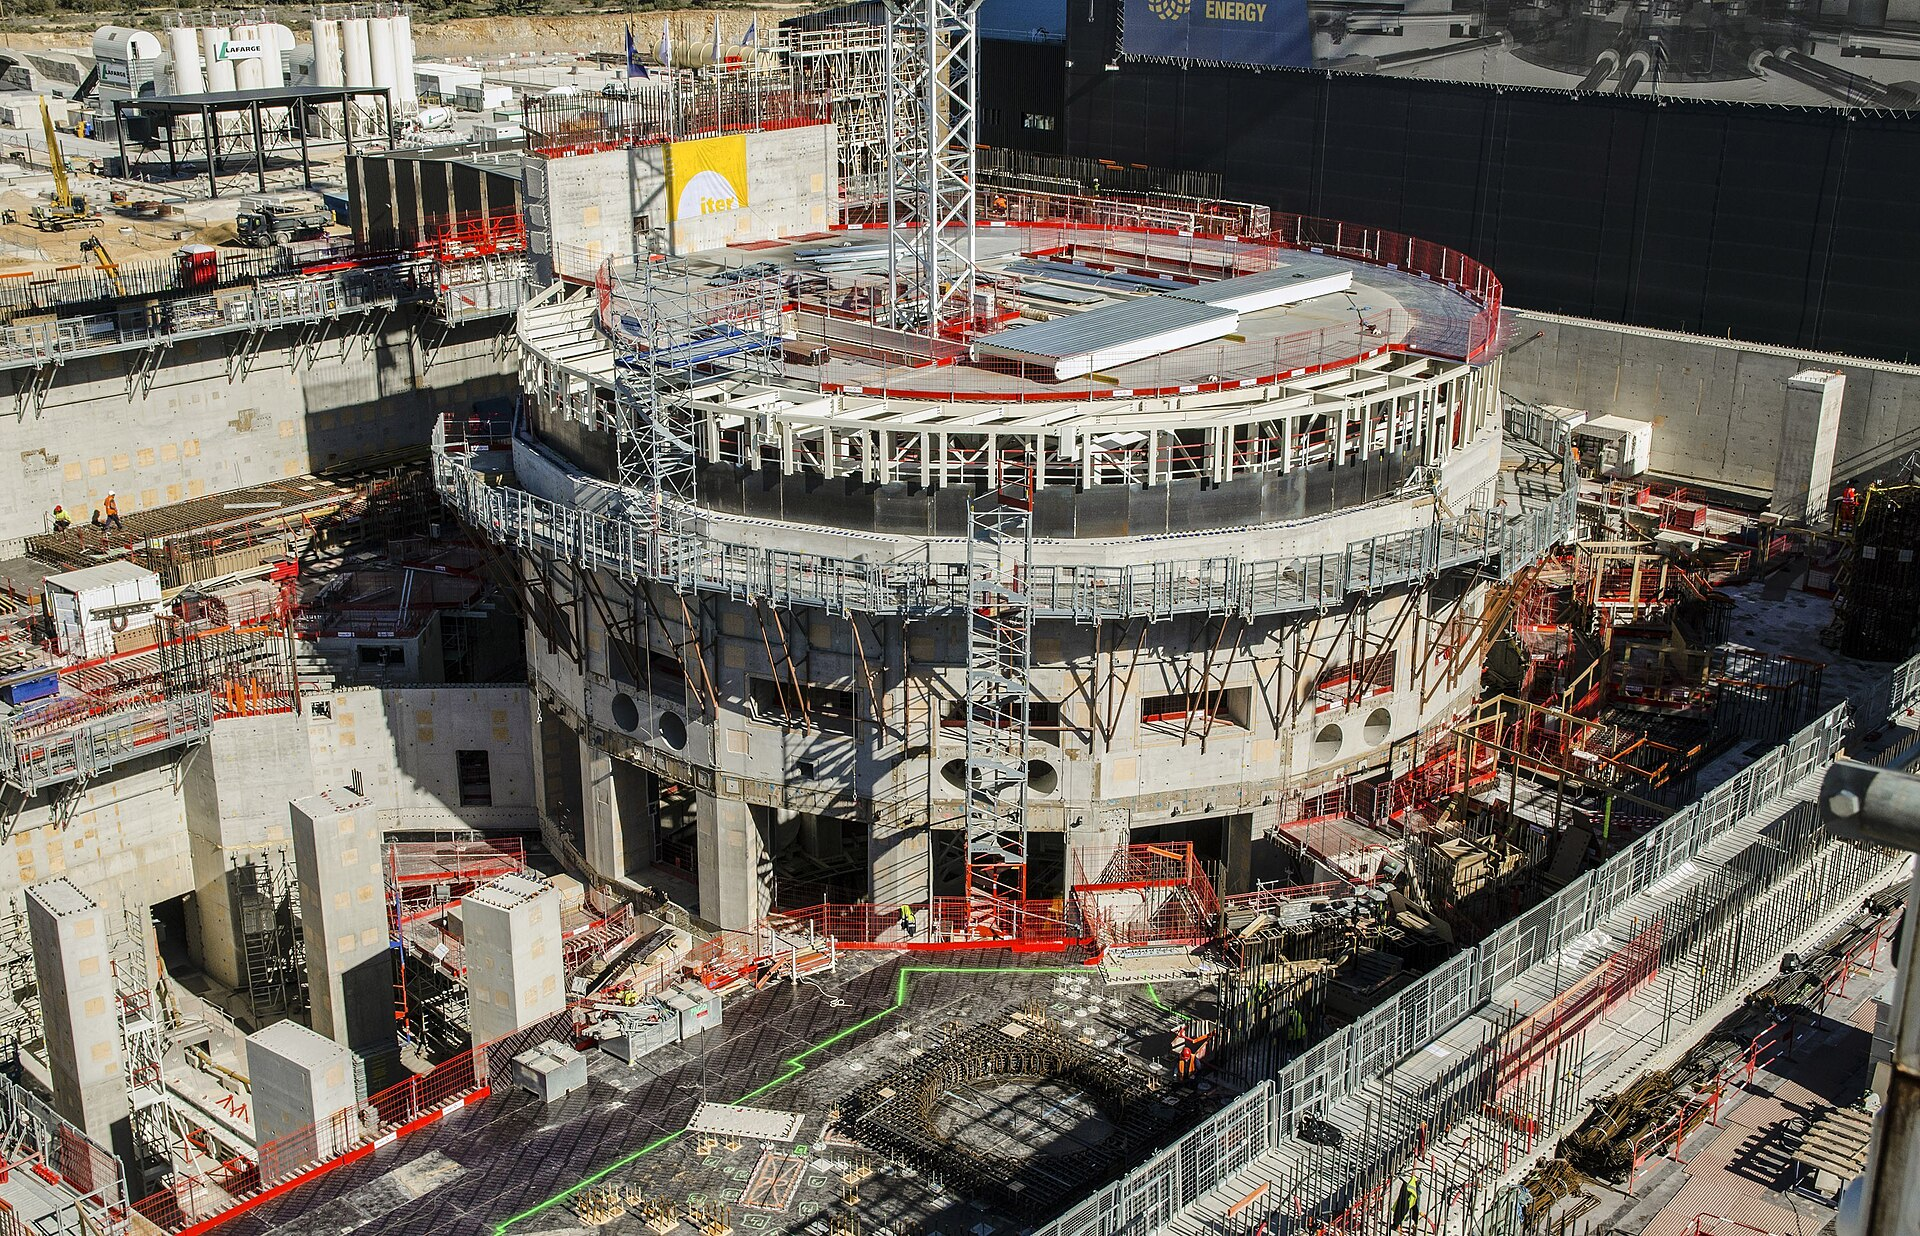
\includegraphics[width=0.72\textwidth]{../figures/az_iter_complex.jpg}
\caption{正在施工的 ITER 主机厂房（2018 年 4 月）。本附录讲的「系统集成」，在工程上就是这个直径几十米的坑：磁体、真空室、包层、低温与电源管线都要塞进去，而且每一路的接口都在别人的空间里——裕度就是这么被吃掉的。}
\label{fig:photo-appaz2}
\figsource{Cedarstrand / ITER Organization，CC BY 2.0（Wikimedia Commons）}
\end{figure}

\section{为什么需要一个「系统」附录：一台堆不是一个物理量}
\label{sec:app-az-why}

前面各附录分别回答了「约束够不够」「材料撑不撑得住」「燃料够不够」「电怎么出去」，
但一个真正能被设计出来的堆，需要把这些答案\textbf{同时}满足。
这就是\textbf{系统集成}：不是把各章结论相加，而是找一个\textbf{自洽的设计点}——
在这个点上，功率平衡、约束时间、密度与比压极限、热流、材料寿命、氚自持与
电功率全部同时成立，而且每一项都留有\textbf{设计裕度}。

先看本附录工作点的系统账（全部取自相邻附录，口径一致）：

\begin{table}[htbp]
\centering
\small
\setlength{\tabcolsep}{4pt}
\begin{tabular}{p{4.4cm}p{2.8cm}p{4.0cm}}
\toprule
项目 & 数值 & 来源口径 \\
\midrule
聚变功率 & $556.5$ MW & 工作点 D1 \\
$\alpha$ 自加热功率 & $111.325$ MW & 中子份额 $79.99545\%$ \\
中子功率 & $445.175$ MW & 附录 Z/AV \\
辐射损失 & $27.8322$ MW（$5.00129\%\,P_\mathrm{fus}$） & 附录 X \\
加热与电流驱动 & $50$ MW & 本附录声明 \\
低温与厂用电 & $13.4157+8.0$ MW & 附录 AM/AR \\
环流功率 & $71.4157$ MW & $P_\mathrm{CD}+P_\mathrm{cryo}+P_\mathrm{plant}$ \\
\bottomrule
\end{tabular}
\caption{系统账的起点：本书工作点的功率清单（与相邻附录同口径）。}
\label{tab:app-az-books}
\end{table}

\textbf{系统集成的第一条纪律是「口径一致」}：$P_\mathrm{fus}$ 用的是热功率还是电功率？
$Q$ 的分母里算不算低温与厂用电？辐射损失算不算在输运损失里？
口径不统一，后面的自洽解就会在几倍的误差上打转。

\begin{tip}{系统集成不是把各章加总，而是找一个自洽点}{tip-app-az-why}
一个常见的误区是「把各附录最乐观的数拼起来」——约束取最好的定标、
密度取 Greenwald 极限、材料取最耐辐照的钢。这样拼出来的设计点
几乎总是不自洽：密度一高，$\beta_N$ 就超限；比压一高，$q_{95}$ 就掉到下限以下；
电流驱动功率一升，再循环功率就把净电吃光。
系统集成的价值恰恰在于\textbf{把「同时成立」这四个字量化}。
\end{tip}

{\footnotesize
\textbf{出处：}0-D 系统账的写法、口径一致性的要求与设计点概念参照
Stacey 的聚变堆设计教材、Freidberg 的等离子体物理与聚变能教材，
以及 ITER/DEMO 设计研究的公开技术文件；本书只借账目结构与判据，
不复制其系统码程序、设计参数表与运行方案。
}

\section{0-D 功率平衡：Q、增益与再循环}
\label{sec:app-az-power}

把等离子体看成一个「零维盒子」：体积 $V$、密度 $n$、温度 $T$，
聚变产生 $\alpha$ 功率自加热，辅助加热补足差额，输运把能量带走。
在这个口径下，两个最常用的增益定义是

\begin{equation}
Q_\mathrm{pl}=\frac{P_\mathrm{fus}}{P_\mathrm{CD}}
=\frac{556.5}{50}=11.13,
\qquad
Q_\mathrm{eng}=\frac{P_\mathrm{fus}}{P_\mathrm{CD}+P_\mathrm{cryo}+P_\mathrm{plant}}
=\frac{556.5}{71.4157}=7.7924.
\label{eq:app-az-q}
\end{equation}

注意两者的分母差别：$Q_\mathrm{pl}$ 只算加热与电流驱动，
$Q_\mathrm{eng}$ 还要算低温与厂用电。\textbf{附录 AR 给出的工程增益是 $2.02345$}，
因为那里的分母还包含变换损耗与全部电耗——同一个物理量在不同口径下
可以差三倍多，写论文时必须写清分母。

零维功率平衡本身是一条很简单的方程：注入的功率必须等于被输运带走的功率，

\begin{equation}
P_\mathrm{alpha}+P_\mathrm{CD}
=\frac{3nk_BTV}{\tau_E},
\qquad
3nk_BTV=367.759\ \mathrm{MJ},
\label{eq:app-az-balance}
\end{equation}

其中 $3nk_BTV$ 是等离子体的总储能（密度、温度、体积三项都取工作点值）。
于是\textbf{约束时间被反过来确定}：

\begin{equation}
\tau_E=\frac{3nk_BTV}{P_\mathrm{alpha}+P_\mathrm{CD}}
=\frac{367.759\ \mathrm{MJ}}{161.325\ \mathrm{MW}}=2.27962\ \mathrm{s}.
\label{eq:app-az-taue}
\end{equation}

这个 $2.27962$ s 不是测量值，而是\textbf{设计要求}：如果实验只能做到它的一半，
就必须把辅助加热从 $50$ MW 提到

\begin{equation}
P_\mathrm{CD}^{(\tau_E/2)}=\frac{3nk_BTV}{\tau_E/2}-P_\mathrm{alpha}=211.325\ \mathrm{MW},
\label{eq:app-az-half}
\end{equation}

四倍多的加热功率，直接把 $Q_\mathrm{pl}$ 从 $11.13$ 压到 $2.6$ 量级。
反过来，若完全不用辅助加热（点火），需要的约束时间是 $3.30348$ s。
\textbf{这三个数放在一起就说明了聚变设计的核心张力：约束的每一点余量，
都要用加热功率（也就是再循环电功率）去换。}

\begin{table}[htbp]
\centering
\small
\setlength{\tabcolsep}{4pt}
\begin{tabular}{p{4.6cm}p{2.8cm}p{3.6cm}}
\toprule
量 & 符号 & 数值 \\
\midrule
等离子体增益 & $Q_\mathrm{pl}$ & $11.13$ \\
工程增益（简化分母） & $Q_\mathrm{eng}$ & $7.7924$ \\
需要输运带走的功率 & $P_\mathrm{alpha}+P_\mathrm{CD}$ & $161.325$ MW \\
等离子体储能 & $3nk_BTV$ & $367.759$ MJ \\
自洽约束时间 & $\tau_E$ & $2.27962$ s \\
约束减半所需的加热 & $P_\mathrm{CD}$ & $211.325$ MW \\
点火所需约束时间 & $\tau_E(Q=0)$ & $3.30348$ s \\
\bottomrule
\end{tabular}
\caption{0-D 功率平衡的完整换算：从储能到约束时间，再到加热需求。}
\label{tab:app-az-power}
\end{table}

\begin{tip}{Q 是定义，不是物理定律}{tip-app-az-q}
$Q_\mathrm{pl}=11.13$ 看起来很漂亮，但它只是「聚变功率除以加热功率」。
真正决定电厂能不能发电的是\textbf{再循环功率}：加热、电流驱动、低温、
厂用电都要从发电机端扣掉。工程上更关心的是
$Q_\mathrm{eng}$ 以及最终的净电效率——这也是为什么附录 AR 把
「每 1 MW 净电对应 $3.73551$ MW 聚变功率」单独算了一遍。
\end{tip}

{\footnotesize
\textbf{出处：}0-D 功率平衡、$Q_\mathrm{pl}$ 与 $Q_\mathrm{eng}$ 的定义、
点火与辅助加热的关系参照 Stacey、Freidberg 的教材与 Wesson 的
托卡马克教材；本书只借方程形式与量级，不复制其运行场景与参数表。
}

\section{自洽解：把 0-D 方程迭代到收敛}
\label{sec:app-az-solve}

上面的 $\tau_E=2.27962$ s 是用固定密度温度算出来的。真实的设计流程是
\textbf{反过来的}：给定加热功率与装置尺寸，用经验定标算约束时间，
再用功率平衡算温度，再用温度算聚变功率，如此循环直到收敛。
本附录用 IPB98(y,2) 型定标做量级估计：

\begin{equation}
\tau_E^\mathrm{IPB}=0.145\,I_p^{0.93}B^{0.15}P^{-0.69}n^{0.41}
(2a)^{0.19}R^{1.97}=3.27992\ \mathrm{s}
\label{eq:app-az-ipb}
\end{equation}

（$I_p$ 用 MA、$B$ 用 T、$P$ 用 MW、$n$ 用 $10^{20}\ \mathrm{m^{-3}}$、
长度用 m）。它与自洽要求 $2.27962$ s 的比值是 $1.4388$，
也就是说\textbf{约束裕度约 $1.44$ 倍}——等价地说，需要达到的
$H$ 因子（实验约束时间与定标之比）只有

\begin{equation}
H=\frac{\tau_E}{\tau_E^\mathrm{IPB}}=\frac{2.27962}{3.27992}=0.695023,
\label{eq:app-az-h}
\end{equation}

低于 $1$，属于「定标已经够用」的乐观情况。反过来说，
\textbf{如果实验只能做到定标值的 $0.8$ 倍}，则需要的辅助加热只有
$28.8307$ MW——比 $50$ MW 还少，因为更差的约束对应更高的加热功率需求，
而更高的加热功率又让\emph{功率平衡}更容易满足……这句话看起来矛盾，
其实是 0-D 反解的特性：$P_\mathrm{CD}$ 出现在分子（加热）也出现在分母（定标退化）。
\textbf{真正的自洽解必须同时收敛温度和聚变功率}，这正是系统码要做的事。

迭代过程本身的收敛速度也值得算一笔：若每步把相对残差压低 $10$ 倍，
从 $1$ 降到 $10^{-3}$ 只需约 $3$ 次迭代。\textbf{困难不在迭代次数，
而在每次迭代里用哪个定标、哪些量固定}——固定 $\beta_N$ 与固定密度
会得到完全不同的收敛路径，这也是设计点不唯一的原因。

\begin{table}[htbp]
\centering
\small
\setlength{\tabcolsep}{4pt}
\begin{tabular}{p{4.8cm}p{2.8cm}p{3.4cm}}
\toprule
量 & 符号 & 数值 \\
\midrule
IPB98(y,2) 定标约束时间 & $\tau_E^\mathrm{IPB}$ & $3.27992$ s \\
自洽要求 & $\tau_E$ & $2.27962$ s \\
约束裕度 & $\tau_E^\mathrm{IPB}/\tau_E$ & $1.4388$ \\
所需 $H$ 因子 & $H$ & $0.695023$ \\
$0.8$ 倍定标时的加热需求 & $P_\mathrm{CD}$ & $28.8307$ MW \\
迭代收敛（$10$ 倍/步） & --- & 约 $3$ 次 \\
\bottomrule
\end{tabular}
\caption{自洽迭代：定标、约束裕度、所需 $H$ 因子与加热需求。}
\label{tab:app-az-solve}
\end{table}

\begin{tip}{自洽解没有唯一答案，只有「哪一套假设」}{tip-app-az-solve}
同一套工程约束下，固定 $\beta_N$、固定密度、固定 $H$ 因子会给出三个
不同的设计点。系统码报告的从来不是「唯一解」，而是\textbf{在给定假设下
彼此自洽的一组解}。读设计报告时，第一件事就是找它固定了哪些量——
这比记住任何单个数字都重要。
\end{tip}

{\footnotesize
\textbf{出处：}IPB98(y,2) 约束定标的形式与指数、$H$ 因子口径、
0-D 自洽迭代流程参照 ITER 定标工作、Stacey 与 Freidberg 的教材；
本书只借定标形式与迭代结构，不复制其拟合系数表、系统码与运行方案。
\section{工作窗与三重积：可用区是怎么围出来的}
\label{sec:app-az-window}
}

功率平衡给出的是「需要多少约束时间」，但装置能在哪个密度、比压与安全因子
区间里运行，是由一组\textbf{经验极限}决定的。最常用的三条是密度极限、
比压极限与安全因子下限。

\textbf{Greenwald 密度极限}把可用的线平均密度与等离子体电流绑在一起：

\begin{equation}
n_G=\frac{I_p}{\pi a^2}
=\frac{15\ \mathrm{MA}}{\pi\times(2.0\ \mathrm{m})^2}
=1.19366\times10^{20}\ \mathrm{m^{-3}},
\qquad
\frac{n}{n_G}=0.837758=83.7758\%
\label{eq:app-az-greenwald}
\end{equation}

密度裕度 $1.19366$——只剩不到 $20\%$。

\textbf{比压}是等离子体压强与磁压之比，\textbf{归一化比压} $\beta_N$ 还乘上
尺寸与电流，便于跨装置比较：

\begin{equation}
\beta=\frac{2\mu_0 nk_BT}{B^2}
=\frac{2\times4\pi\times10^{-7}\times147304}{(5.3)^2}
=0.0131796=1.31796\%,
\label{eq:app-az-beta}
\end{equation}

\begin{equation}
\beta_N=\beta\,[\%]\times\frac{a B}{I_p}
=1.31796\times\frac{2.0\times5.3}{15}=0.93136
\quad(\%\cdot\mathrm{m}\cdot\mathrm{T/MA}),
\qquad
\text{裕度}=\frac{3.0}{0.93136}=3.2211.
\label{eq:app-az-betan}
\end{equation}

\textbf{安全因子}决定磁流体稳定性：圆柱近似给出

\begin{equation}
q_{95}^\mathrm{cyl}=\frac{5a^2B}{RI_p}
=\frac{5\times4\times5.3}{6.2\times15}=1.13978,
\qquad
q_{95}=2.6\,q_{95}^\mathrm{cyl}=2.96344,
\label{eq:app-az-q95}
\end{equation}

其中 $2.6$ 是成形因子（拉长与三角形变）。$q_{95}$ 的下限取 $2.0$，
裕度 $1.48172$。

三条极限与功率平衡一起，把「可用区」围成 $n$--$T$ 图上的一个窗口。
窗口里最常被引用的一条综合指标是\textbf{三重积}：

\begin{equation}
\begin{aligned}
n T \tau_E&=1.0\times9.194\times2.27962=20.9588\ (10^{20}\ \mathrm{keV\,s\,m^{-3}}),\\
\text{相对点火判据 }&5\times10^{21}\ \text{的裕度}=4.19176 .
\end{aligned}
\label{eq:app-az-triple}
\end{equation}

\begin{table}[htbp]
\centering
\small
\setlength{\tabcolsep}{4pt}
\begin{tabular}{p{4.4cm}p{2.6cm}p{2.4cm}p{2.6cm}}
\toprule
限制 & 工作点值 & 限值 & 裕度 \\
\midrule
Greenwald 密度 & $0.837758\,n_G$ & $n_G$ & $1.19366$ \\
归一化比压 & $\beta_N=0.93136$ & $3.0$ & $3.2211$ \\
安全因子 & $q_{95}=2.96344$ & $2.0$ & $1.48172$ \\
三重积 & $20.9588$ & $50$ & $4.19176$ \\
\bottomrule
\end{tabular}
\caption{工作窗的三条经验极限与三重积：工作点值、限值与裕度。}
\label{tab:app-az-window}
\end{table}

\begin{tip}{三重积是三条极限围出来的，不是一条公式}{tip-app-az-triple}
$nT\tau_E$ 常被当成「聚变性能的单一指标」，但它只是一个乘积：
密度被 Greenwald 限住、比压被 $\beta_N$ 限住、安全因子被 $q_{95}$ 限住，
约束时间由输运决定。\textbf{把三条极限画在同一张 $n$--$T$ 图上，
交集才是可用区}——只看三重积容易得出「只要把三个量都乘以 2 就行」的错误结论。
\end{tip}

{\footnotesize
\textbf{出处：}Greenwald 密度极限、$\beta_N$ 口径、$q_{95}$ 圆柱近似与
成形因子的量级、三重积与点火判据参照 Freidberg、Wesson 的教材与
ITER 设计研究的公开技术文件；本书只借经验判据的形式与量级，
不复制其数据库、定标拟合与运行限制表。
}

\section{设计裕度：怎么定义、怎么分配}
\label{sec:app-az-margin}

\textbf{设计裕度}（design margin）的定义很朴素：限值与工作点之比，

\begin{equation}
M=\frac{\text{限值}}{\text{工作点值}},
\qquad
M>1\ \text{才算可用}.
\label{eq:app-az-margin}
\end{equation}

把前面各节的结果汇总成一张裕度表，就得到本附录最有用的输出：

\begin{table}[htbp]
\centering
\small
\setlength{\tabcolsep}{4pt}
\begin{tabular}{p{3.8cm}p{3.4cm}p{2.6cm}p{2.2cm}}
\toprule
裕度项 & 限值 / 工作点 & 裕度 & 类别 \\
\midrule
密度 & $n_G$ / $0.837758\,n_G$ & $1.19366$ & 物理 \\
归一化比压 & $3.0$ / $0.93136$ & $3.2211$ & 物理 \\
安全因子 & $q_{95}$ / $2.0$ & $1.48172$ & 物理 \\
约束 & $\tau_E^\mathrm{IPB}$ / $\tau_E$ & $1.4388$ & 物理 \\
材料剂量 & $50$ / $44.5634$ dpa & $1.122$ & 工程 \\
氚自持 & $1.05$ / $1.01802$ & $1.03141$ & 工程 \\
可用率 & $0.821918$ / $0.780822$ & $1.05263$ & 工程 \\
\bottomrule
\end{tabular}
\caption{七项裕度的汇总：三项工程裕度比四项物理裕度都紧。}
\label{tab:app-az-margin}
\end{table}

三个结论值得单独说：

\begin{itemize}
\item \textbf{最紧的不是物理，而是工程}：最小裕度是氚自持的 $1.03141$，
  其次是可用率 $1.05263$ 与材料剂量 $1.122$。这三项任何一项失守，
  整个设计点就不成立——而它们的误差往往来自工程实现，不是等离子体物理。
\item \textbf{六项低于 $1.5$}：只有 $\beta_N$（$3.2211$）高于常用的
  「不低于 $1.5$」门槛。把最小裕度再除以 $1.2$ 的安全系数，
  就掉到 $0.859512$——\textbf{低于 1，意味着这个设计点没有余量}。
\item \textbf{裕度不能简单相乘}：七项相乘是 $9.98512$，看似很大；
  但如果要求每一项独立留 $1.2$ 的工程裕度，$1.2^7=3.58318$，
  等于把整个设计点的性能压掉一大截。\textbf{裕度是「分配」问题，
  不是「越多越好」问题}。
\end{itemize}

\begin{tip}{最小裕度决定生死，平均裕度决定成本}{tip-app-az-margin}
设计评审里最危险的一句话是「平均裕度还有 $1.4$」。
串联系统里决定成败的是\textbf{最小}那一项（木桶效应）；
而平均裕度只影响造价与复杂度。
本工作点的教训很典型：等离子体物理给足了余量，
卡住设计点的却是氚自持、可用率与材料寿命这三项工程指标。
\end{tip}

{\footnotesize
\textbf{出处：}设计裕度的定义与分配、木桶效应式的串联判据、
物理裕度与工程裕度的分类参照系统工程的通用做法与
聚变设计研究的公开技术文件；本书只借判据形式，
不复制其裕度分配表与评审程序。
}

\section{灵敏度分析：哪个参数最值钱}
\label{sec:app-az-sensitivity}

有了自洽解，下一个问题自然是「改哪个参数最划算」。
标准工具是\textbf{对数灵敏度}：

\begin{equation}
S_x=\frac{\partial\ln y}{\partial\ln x}
=\frac{x}{y}\frac{\partial y}{\partial x},
\label{eq:app-az-sens}
\end{equation}

它表示「$x$ 提高 $1\%$，$y$ 提高 $S_x\%$」。对聚变功率，
用 $P_\mathrm{fus}\propto n^2\langle\sigma v\rangle V$ 逐项求导即得：

\begin{equation}
\begin{aligned}
&S_n=2,\qquad S_T=2\ (\langle\sigma v\rangle\propto T^2\ \text{在}\ 10\ \mathrm{keV}\ \text{附近}),\\
&S_B=4\ (\text{固定}\ \beta\ \text{时}\ n\propto B^2),\qquad S_R=3\ (V\propto R^3).
\end{aligned}
\label{eq:app-az-sens2}
\end{equation}

\begin{table}[htbp]
\centering
\small
\setlength{\tabcolsep}{4pt}
\begin{tabular}{p{4.2cm}p{2.4cm}p{5.0cm}}
\toprule
旋钮 & 灵敏度 & 说明 \\
\midrule
磁场 $B$ & $S_B=4$ & 固定比压时 $n\propto B^2$，最值钱 \\
大半径 $R$ & $S_R=3$ & 体积按立方增长（造价也按立方涨） \\
密度 $n$ & $S_n=2$ & 但会撞 Greenwald 极限 \\
温度 $T$ & $S_T=2$ & 在 $10$ keV 附近 $\langle\sigma v\rangle\propto T^2$ \\
约束时间 $\tau_E$ & $S_\tau=1$ & 对 $Q_\mathrm{pl}$ 线性 \\
加热功率 $P_\mathrm{CD}$ & $S=-1$ & 同时是分母与电耗，最贵 \\
\bottomrule
\end{tabular}
\caption{对数灵敏度一览：哪个旋钮值钱、哪个最贵。}
\label{tab:app-az-sens}
\end{table}

几个可以直接引用的例子：

\begin{itemize}
\item $B$ 从 $5.3$ 提到 $5.8$ T（$+9.43396\%$），聚变功率变 $1.4342$ 倍；
\item $R$ 从 $6.2$ 提到 $6.8$ m，聚变功率变 $1.31932$ 倍（但造价涨更多）；
\item 约束时间提高 $10\%$，维持同一 $\tau_E$ 所需的加热功率降到 $35.3341$ MW，
  也就是少花约 $15$ MW 的电；
\item 定标指数 $-0.69$ 的含义：$P_\mathrm{loss}$ 提高 $10\%$，
  $\tau_E^\mathrm{IPB}$ 降到 $0.936352$ 倍，为保持同一性能
  $H$ 因子需要提高 $1.06797$ 倍——\textbf{这就是「功率越高约束越差」的定量表述}。
\end{itemize}

\begin{tip}{灵敏度告诉你「往哪儿投钱」，裕度告诉你「还差多少」}{tip-app-az-sens}
两者要一起看：$S_B=4$ 说明提高磁场最划算，但磁场的上限由
超导材料决定（附录 AM 的临界电流与失超保护）；$S_n=2$ 说明加密度有效，
但密度裕度只剩 $1.19366$。\textbf{灵敏度只回答「斜率」，
裕度回答「距离」}——设计优化永远是「斜率大的方向上还有多少距离」。
\end{tip}

{\footnotesize
\textbf{出处：}对数灵敏度的定义与聚变功率对各参数的灵敏度指数、
约束定标指数的解读参照 Freidberg 的教材与
系统码灵敏度分析的公开文献；本书只借方法，
不复制其灵敏度矩阵与优化结果。
\section{集成检查清单：从 0-D 到工程约束}
\label{sec:app-az-checklist}
}

把前面六节串起来，就得到一张可以照着走的\textbf{集成检查清单}。
每一项都是一条不等式，全部满足才算设计点成立：

\begin{equation}
\underbrace{\frac{n}{n_G}\le1}_{\text{密度}}
\wedge\underbrace{\frac{\beta_N}{3}\le1}_{\text{比压}}
\wedge\underbrace{\frac{2.0}{q_{95}}\le1}_{\text{稳定性}}
\wedge\underbrace{\frac{\tau_E}{\tau_E^\mathrm{IPB}}\le1}_{\text{约束}}
\wedge\underbrace{\frac{t\,D_\mathrm{fpy}}{50}\le1}_{\text{材料}}
\wedge\underbrace{\frac{c_\mathrm{He}}{600}\le1}_{\text{氦}}
\wedge\underbrace{\frac{1.01802}{\mathrm{TBR}}\le1}_{\text{氚}}
\wedge\underbrace{\frac{t}{t_\mathrm{creep}}\le1}_{\text{蠕变}} .
\label{eq:app-az-checklist}
\end{equation}

\noindent 本工作点对前七项的检查结果全部通过（最小裕度 $1.03141$）；
第八项（蠕变）在附录 AY 里算过，余量 $2.28154$ 倍。

\textbf{电账}是清单里最容易被忽略的一项。发电端与净电端分开算：

\begin{equation}
P_\mathrm{gross}=\eta_\mathrm{th}P_\mathrm{fus}=0.40\times556.5=222.6\ \mathrm{MW},
\qquad
P_\mathrm{net}=P_\mathrm{gross}-P_\mathrm{CD}-P_\mathrm{cryo}-P_\mathrm{plant}=151.184\ \mathrm{MW},
\label{eq:app-az-net}
\end{equation}

净电效率 $27.167\%$；若再扣掉变换损耗 $2.20873$ MW（附录 AR 的口径），
就是附录 AR 给出的 $26.7701\%$。\textbf{同一个电厂，两篇文章可能报出
$27.2\%$ 与 $26.8\%$ 两个效率}——差别只在是否把变换损耗算进去。

\textbf{电流驱动}决定了「稳态」两个字能不能写：

\begin{equation}
I_\mathrm{bs}=0.30\times15=4.5\ \mathrm{MA},
\qquad
I_\mathrm{CD}=15-4.5=10.5\ \mathrm{MA},
\qquad
P_\mathrm{CD}^\mathrm{need}=\frac{10.5}{0.30}=35\ \mathrm{MW},
\label{eq:app-az-cd}
\end{equation}

需要的驱动功率 $35$ MW 小于声明的 $50$ MW，\textbf{说明电流驱动不是最紧的一项}。

\textbf{热流}是精简的检验：把输运功率减去辐射，再摊到偏滤器湿面积上，

\begin{equation}
P_\mathrm{sep}=P_\mathrm{alpha}+P_\mathrm{CD}-P_\mathrm{rad}=133.493\ \mathrm{MW},
\qquad
q_\mathrm{peak}=\frac{P_\mathrm{sep}}{A_\mathrm{wet}}=\frac{133.493}{3}=44.4976\ \mathrm{MW\,m^{-2}},
\label{eq:app-az-heatflux}
\end{equation}

$44.4976\ \mathrm{MW\,m^{-2}}$ 远高于常规偏滤器的稳态承受能力
（这也是为什么必须引入脱靶与辐射偏滤器——见附录 N）。

\begin{table}[htbp]
\centering
\small
\setlength{\tabcolsep}{4pt}
\begin{tabular}{p{4.0cm}p{3.6cm}p{3.8cm}}
\toprule
检查项 & 判据 & 本工作点结果 \\
\midrule
密度 & $n/n_G\le1$ & $0.837758$，通过 \\
比压 & $\beta_N/3\le1$ & $0.310453$，通过 \\
稳定性 & $2.0/q_{95}\le1$ & $0.674891$，通过 \\
约束 & $\tau_E/\tau_E^\mathrm{IPB}\le1$ & $0.695023$，通过 \\
材料 & $5D_\mathrm{fpy}/50\le1$ & $0.891268$，通过（最紧之一） \\
氚 & $1.01802/\mathrm{TBR}\le1$ & $0.969543$，通过（最紧） \\
可用率 & $0.780822/0.821918\le1$ & $0.95$，通过 \\
电流驱动 & $P_\mathrm{CD}^\mathrm{need}\le P_\mathrm{CD}$ & $35\le50$ MW，通过 \\
热流 & $q_\mathrm{peak}\le q_\mathrm{limit}$ & $44.4976$ vs $10$ 量级，\textbf{不通过} \\
\bottomrule
\end{tabular}
\caption{集成检查清单：八项通过、一项不通过（热流），这就是设计需求。}
\label{tab:app-az-checklist}
\end{table}

\begin{tip}{清单全部通过只是及格线}{tip-app-az-checklist}
八项通过、一项不通过（热流）是典型的真实结果：
\textbf{系统集成的输出不是「设计成功」，而是「下一个要解决的问题是什么」}。
本工作点给出的答案是热流——这也解释了为什么现代托卡马克设计里
偏滤器与辐射偏滤器（附录 N）会成为独立的研究方向。
清单的另一个用处是\textbf{追踪最小裕度随时间的变化}：
设计迭代过程中，某一项裕度突然掉到 $1.05$ 以下，
就意味着设计的重心要转移过去。
\end{tip}

{\footnotesize
\textbf{出处：}集成检查清单的判据集合、电账与电流驱动账的口径、
偏滤器热流量级参照 Stacey 的教材、ITER/DEMO 设计研究的公开技术文件
与附录 N 的脱靶口径；本书只借清单结构，不复制其设计点与裕度分配。
}

\section{估算练习}
\label{sec:app-az-problems}

\textbf{练习 1} 若把加热功率从 $50$ MW 翻倍到 $100$ MW，
$Q_\mathrm{pl}$ 与 $Q_\mathrm{eng}$ 各变成多少？

\textbf{解答 1} $Q_\mathrm{pl}=556.5/100=5.565$（下降 $2$ 倍）；
$Q_\mathrm{eng}=556.5/(100+13.4157+8.0)=4.58343$。
\textbf{增益对加热功率是 $1/x$ 的关系}，翻倍加热就折半增益。

\textbf{练习 2} 若把密度提到 $1.2\times10^{20}\ \mathrm{m^{-3}}$，
密度与比压裕度各是多少？

\textbf{解答 2} $n/n_G=1.2/1.19366=1.00531$，\textbf{已经越过 Greenwald 极限}；
$\beta_N=0.93136\times1.2=1.11763$（裕度降到 $2.68425$），
密度裕度变成 $0.994718$——\textbf{低于 1，即设计点不成立}。

\textbf{练习 3} 若约束定标只能保证 $2.0$ s，需要多少加热功率？$Q_\mathrm{pl}$ 多少？

\textbf{解答 3} $P_\mathrm{CD}=3nk_BTV/2.0-P_\mathrm{alpha}=72.5547$ MW，
$Q_\mathrm{pl}=556.5/72.5547=7.67007$。约束从 $2.28$ s 掉到 $2.0$ s，
加热需求涨 $45.1094\%$，增益掉 $31.087\%$。

\textbf{练习 4} 若磁场从 $5.3$ 降到 $5.0$ T，聚变功率与 $\beta_N$ 怎么变？

\textbf{解答 4} 固定比压时 $P_\mathrm{fus}\propto B^4$：
$(5.0/5.3)^4=0.792094$，即掉约 $20.7906\%$；
而同一密度下 $\beta_N\propto1/B^2$ 会升高 $(5.3/5.0)^2=1.1236$ 倍——
\textbf{降磁场既减功率又吃比压裕度}，是双输。

\textbf{练习 5} 若 TBR 只有 $1.02$，氚自持的裕度是多少？五年能净攒多少氚？

\textbf{解答 5} 相对下限 $1.01802$ 的裕度是 $1.02/1.01802=1.00194$
（比声明值 $1.05$ 紧得多）；以附录 AV 的 $89.7384$ g/day 消耗计，
五年净盈余 $(1.02-1.01802)\times89.7384\times5=0.88841$ kg。
\textbf{自持裕度只有 $0.194\%$，任何一个提取环节的效率损失都会把它吃掉。}

\textbf{练习 6} 若三个最紧的裕度分别是 $1.8$、$1.5$、$1.2$，
整体裕度是多少？为什么不能这样算？

\textbf{解答 6} 乘积是 $3.24$。但\textbf{串联系统的整体裕度不是乘积，
而是最小值}——决定成败的是 $1.2$ 那一项。乘积只说明「平均下来还有余地」。

\section{来源、分级与版权说明}
\label{sec:app-az-source}

\begingroup\small
本附录的数值全部由 \texttt{tools/\allowbreak{}calc/\allowbreak{}appAZ\_calc.py} 复算（输出
\texttt{tools/\allowbreak{}calc/\allowbreak{}appAZ\_calc.txt}），工作点与附录 M/S/U/V/W/X/AK/AP/AV/AX/AY 一致，
工程侧输入（$P_\mathrm{CD}$、$P_\mathrm{cryo}$、$P_\mathrm{plant}$、
$\eta_\mathrm{th}$、辐射损失、TBR 与下限、可用率、5 年剂量、
自举份额、电流驱动效率、$\beta_N$ 与 $q_{95}$ 限值）都是\textbf{声明输入}，
量级取自下列公开来源；本附录只借公式形式与判据，
\textbf{不复制}任何成段文字、原图、系统码程序或设计参数表。

\begin{table}[htbp]
\centering
\small
\setlength{\tabcolsep}{4pt}
\begin{tabular}{p{5.0cm}p{5.0cm}p{2.8cm}}
\toprule
主题 & 借鉴来源 & 本书用法 \\
\midrule
0-D 功率平衡与设计点 & Stacey, \emph{Fusion: An Introduction...}；Freidberg, \emph{Plasma Physics and Fusion Energy} & 方程与判据形式 \\
经验极限（$n_G$、$\beta_N$、$q_{95}$） & Greenwald 等 (2002)；Wesson, \emph{Tokamaks} & 极限形式与量级 \\
约束定标与 $H$ 因子 & ITER Physics Basis（IPB98(y,2)） & 定标形式与指数 \\
系统码与灵敏度分析 & Kovari 等（PROCESS）等公开系统码文献 & 流程与灵敏度方法 \\
电账与再循环功率 & 附录 AR 与 ITER/DEMO 公开设计文件 & 口径与量级 \\
热流与脱靶 & 附录 N 与偏滤器公开设计文件 & 量级判据 \\
\bottomrule
\end{tabular}
\caption{本附录的借鉴来源、分级与用途（逐条注明，不复制原文）。}
\label{tab:app-az-source}
\end{table}

\textbf{分级说明}：AZ.1--AZ.4 的账目与工作窗计算是\textbf{可复算的量级估算}，
任何读者都能用声明输入重算；AZ.5--AZ.7 的裕度与灵敏度是\textbf{设计方法}，
给出的是「哪一项最紧、哪个旋钮最值钱」的判断，不能替代系统码与工程评审。
本附录\textbf{不复制}：任何教材的成段文字与原图、系统码源码、
设计参数表与裕度分配表。

\textbf{出处：}本节的来源分级与版权口径依照本书统一的
「借公式与量级、不复制原文」原则；与附录 Z（总账）、AR（电源与储能）、
X（辐射损失）、AV（氚自持）、AP（可用率与更换）、AY（材料寿命）、
N（偏滤器热流）的分工见各节交叉引用。
\endgroup
